\documentclass[12pt,a4paper]{report}
\usepackage[utf8]{inputenc}
\usepackage[top=3.3cm,bottom=3cm,right=3cm,left=3cm]{geometry}
\usepackage{amsmath,amsfonts,amssymb,mathrsfs,tikz,pgfornament}
\pagestyle{empty}
\usepackage{polyglossia}
\setmainlanguage[numerals=maghrib]{arabic}
\setotherlanguage{french}
\newfontfamily\arabicfont[Script=Arabic,Scale=1.2]{Amiri}
\newfontfamily\frenchfont{Times New Roman}
\def\z~#1~#2~#3~#4~#5~{
\node [rotate=#1]at (#2:#3){\pgfornament[width=#4cm,color=blue]{#5}};
}
\def\s{%
\tikz{
\draw [line width=2pt](-4,0)-|(0,4);
\draw [line width=1pt](-4,0.14)-|(-0.14,4);
\draw [line width=2pt](-4,0.48)-|(-3.2,1.2)arc(-90:0:1)arc(-90:0:1)-|(-0.48,4);
\draw [line width=1pt](-4,0.38)-|(-3.08,1.1)arc(-90:0:1)arc(-90:0:1)-|(-0.38,4);
\draw[line width=6mm,color=white](135:2.8)+(-0.5,-0.5)--+(.5,.5);
\z~90~135~2.1~2.5~54~
\z~180~102~2.93~.8~55~
\z~-90~168~2.93~.8~56~
\z~0~94.5~5~1~67~
\z~90~178.5~5~1~67~
\z~90~91~16~15~83~
\z~90~92~7.5~6~85~
}
}
\def\r{%
\tikz{
\draw [line width=2pt](-4,0)-|(0,4);
\draw [line width=1pt](-4,0.14)-|(-0.14,4);
\draw [line width=2pt](-4,0.48)-|(-3.2,1.2)arc(-90:0:1)arc(-90:0:1)-|(-0.48,4);
\draw [line width=1pt](-4,0.38)-|(-3.08,1.1)arc(-90:0:1)arc(-90:0:1)-|(-0.38,4);
\draw[line width=6mm,color=white](135:2.8)+(-0.5,-0.5)--+(.5,.5);
\z~90~135~2.1~2.5~54~
\z~180~102~2.93~.8~55~
\z~-90~168~2.93~.8~56~
\z~0~94.5~5~1~67~
\z~90~178.5~5~1~67~
}
}
\def\t{
\tikz{\filldraw[rounded corners=5mm,draw=red!50!white,inner color=white,outer color=red](-4.5,-0.1)to[bend right=5](-2,0.5)--(2,.5)to[bend right=5,sharp corners](4.3,0)to[bend left=5](2,-.5)--(-2,-.5)to[bend left=5]cycle;
\filldraw[rounded corners=5mm,draw=red!50!white,inner color=white,outer color=red](4.5,-0.1)to[bend right=5](2,0.5)--(-2,.5)to[bend left=5,sharp corners](-4.3,0)to[bend left=5](-2,-.5)--(2,-.5)to[bend left=5]cycle;}
}
\usetikzlibrary{arrows,shapes}
\parindent=0mm
\begin{document}
وزارة التعلـــيم العــالــي والـبحـث العلــمي
\hfill
\textfrench{Ministre de l'Ensegnement Séperieur}
\\[-5mm]

\hfill\textfrench{et de la recherche scientifique}
\\[-1mm]
المــدرســة العليــا للأســـاتــذة
\hfill
\textfrench{Ecole Normale Supérieur}\\[1mm]
- القـــبة القديـــمة - الجـــزائــر 
\hfill
\textfrench{- Vieux Kouba - Alger}
\\[2mm]
- قـــســم الريــاضــيـات -
\hfill
\textfrench{\textit{
Département de Mathematique
}}
\\\vfill\centering
\begin{tikzpicture}
\node[inner color=white,outer color=violet!50!blue!50,text width=\linewidth,align=center,font=\bfseries\huge,minimum height=3cm,rectangle,rounded corners=4mm,text=violet](1){\textarabic{%
بعض تقنيات المعالجة
}};
\end{tikzpicture}\\[1cm]
مذكرة تخرج لنيل شهادة أستاذ تعليم ثانوي
\\\flushright\vfill
\begin{minipage}{.5\textwidth}
من إعداد:
\\[4mm]
........
\end{minipage}\hfill
\begin{minipage}{.3\textwidth}
تحت إشراف الأستاذ:
\\[4mm]
.......
\end{minipage}\\\vfill
نوقشت من طرف اللجنة:
\\
- الأستاذ .............
\hfill
رئيسا
\\
- الأستاذ ............ 
\hfill
مشرفا
\\
- الأستاذ ..............
\hfill
ممتحنا
\\
\centering
\vfill
السنة الجـــامعية: 2017/2018
\\[.5cm]
دفعة جوان 2018
\\
\begin{tikzpicture}[overlay,remember picture]
\node at ([shift={(-3.6,12.3)}]current page.south east){\s};
\node [rotate=180]at ([shift={(3.6,-12.3)}]current page.north west){\s};
\node [rotate=90]at ([shift={(-3.6,-3.6)}]current page.north east){\r};
\node [rotate=-90]at ([shift={(3.6,3.6)}]current page.south west){\r};
\node [yscale=0.6,scale=0.8]at ([yshift=-1cm]current page.north){\t};
\node [yscale=0.6,scale=0.8]at ([yshift=1cm]current page.south){\t};
\node at ([shift={(0,-5.2cm)}]current page.north) {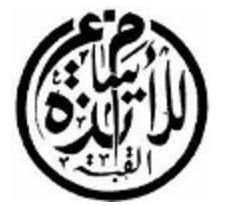
\includegraphics[width=2.cm,height=2.cm]{ens}};
\end{tikzpicture}
\end{document}